\section{Quantization}
\label{sec:quantization}

We apply post-training quantization (PTQ) using Model-Optimizer to quantize the Nemotron 3 Ultra checkpoint to NVFP4 \citep{nvpfp4_ptq_default} for efficient inference on NVIDIA Blackwell GPUs.
The quantization format per operator (GEMM, KVCache, Mamba Cache) is summarized in Table~\ref{tab:quant-recipe}. We begin from a heuristic mixed per-layer precision recipe informed by
Model-Optimizer AutoQuantize\footnote{\url{https://github.com/NVIDIA/Model-Optimizer/tree/main/examples/llm_ptq\#autoquantize}}
sensitivity analysis on Nemotron 3 Super~\citep{nvidia2026nemotron3superopen}.
We then perform ablations over the model's effective
bits per element (BPE) and FP4 weight quantization algorithms to refine this
recipe and select the final operating point.

\begin{table}[!htp]
\centering
\small
\setlength{\tabcolsep}{8pt}
\renewcommand{\arraystretch}{1.3}
\resizebox{\textwidth}{!}{
\begin{tabular}{@{}lcc@{}}
\toprule
\textbf{Layer / Operator} & \textbf{BF16 Baseline} &
\textbf{Quantized Checkpoint Precision} \\
\midrule
Embedding, Output classification layer, MTP layers & BF16 & BF16 \\
MoE routed experts & BF16 & NVFP4 \\
MoE shared experts & BF16 & FP8 per-tensor \\
Mamba mixer linears & BF16 & FP8 per-tensor \\
Attention linears & BF16 & BF16 \\
Latent MoE & BF16 & BF16 \\
Mamba conv1d & BF16 & BF16 \\
KV cache & BF16 & FP8 \\
Mamba SSM cache & FP32 & FP16 with stochastic rounding \\
\bottomrule
\end{tabular}
}
\caption{
Quantization recipe for \ourmodel, mapping each layer or operator
from its BF16 baseline.
}
\label{tab:quant-recipe}
\end{table}


\subsection{Bits per Element Selection}
\label{sec:bpe-sweep}

We selected the model's bits-per-element (BPE) budget empirically, by quantizing a
fixed intermediate checkpoint at a range of BPE settings and scoring each against a
curated suite of evaluations, served through the Nemo Evaluator SDK on vLLM~v0.20.0.
We raised the number of repeats per benchmark to suppress run-to-run variance and
report the averaged pass@1 scores. The suite spans seven benchmarks: coding (SciCode),
scientific reasoning (GPQA~Diamond, HLE, CritPt), instruction following and knowledge
(IFBench, AA-Omniscience), and long-context reasoning (AA-LCR).

The results are summarized in Table~\ref{tab:bpe-sweep}.
Here BPE is best read as a
summary axis over a family of quantization recipes rather than a single tunable knob:
the higher-BPE points correspond to qualitatively different strategies (router-only
quantization, keeping the last MoE layer in BF16, and skipping the top-8 most
sensitive experts), each of which lands at a different effective BPE.

Across the sweep, most capabilities are already saturated at the lowest BPE we tried.
GPQA Diamond, SciCode, HLE,
IFBench, and AA-Omniscience accuracy are flat to within
run-to-run noise across the entire 4.85--7.19 BPE range. The single discriminating
axis is long-context reasoning: AA-LCR improves by $+2.4$ points
at the 4.85~$\rightarrow$~5.03 step and then plateaus (64.2--65.0) all the way
to 7.19~BPE. This step is precisely the introduction of the mixed-FP8 layers on top of
the NVFP4-amax recipe, so the long-context recovery is attributable to those targeted
higher-precision layers rather than to additional bits in general.

Above 5.03~BPE we observe no further gains: increasing the budget to 7.19~BPE
(a 43\% increase in bits) leaves every benchmark unchanged within noise. We therefore
selected \textbf{5.03~BPE} (NVFP4 with mixed-FP8) as the operating point, as it is the
smallest budget that recovers long-context performance while leaving no measurable
quality on the table at higher precision.

We note two caveats in reading Table~\ref{tab:bpe-sweep}. First, CritPt scores sit near
the floor of the benchmark (${\sim}3$--$5\%$) and are non-monotonic across the sweep; we
treat it as noise-dominated rather than a deciding signal here, which is also why the
repeat count was raised. Second, AA-Omniscience's non-hallucination rate mildly favors
the lowest BPE (54.13 at 4.85 versus 51.59 at 5.03); given the magnitude relative to the
other axes we attribute this to variance rather than a genuine precision trade-off.
\label{app:bpe-sweep}

\begin{table}[ht!]
\centering
\small
\setlength{\tabcolsep}{6pt}
\renewcommand{\arraystretch}{1.3}

% requires: booktabs, array, xcolor, colortbl
\begin{tabular}{lr|c >{\columncolor{blue!8}}c c c c}
\toprule
& & \multicolumn{5}{c}{\textbf{Quantization (bits-per-element)}} \\
\cmidrule(lr){3-7}
\textbf{Task} & \textbf{Metric} &
4.85 & \textbf{5.03}$^{\dagger}$ & 5.25 & 5.43 & 7.19 \\
\midrule

\rowcolor{black!5}
\multicolumn{7}{l}{\textbf{Coding}} \\
SciCode & \textit{pass@1 (avg-16), subtask acc} & 43.82 & \textbf{43.88} & 43.45 & 43.27 & 43.44 \\
\midrule

\rowcolor{black!5}
\multicolumn{7}{l}{\textbf{Scientific Reasoning}} \\
GPQA Diamond & \textit{pass@1 (avg-32), sym.\ correct} & 84.66 & 84.33 & \textbf{84.75} & 84.12 & 84.52 \\
HLE & \textit{pass@1, judge correct} & 24.24 & 24.84 & 25.00 & 24.98 & \textbf{25.44} \\
CritPt & \textit{pass@1 (avg-8), accuracy} & 3.04 & 3.93 & \textbf{5.18} & 4.82 & 4.46 \\
\midrule

\rowcolor{black!5}
\multicolumn{7}{l}{\textbf{General}} \\
AA-Omniscience & \textit{pass@1 (avg-20), judge correct} & 29.21 & \textbf{29.75} & 29.18 & 29.29 & 29.00 \\
          & \textit{pass@1 (avg-20), non-hallucination} & \textbf{54.13} & 51.59 & 51.84 & 51.70 & 52.81 \\
IFBench & \textit{pass@1 (avg-8), avg.\ score} & 79.34 & 79.26 & \textbf{79.83} & 79.53 & \textbf{79.83} \\
\midrule

\rowcolor{black!5}
\multicolumn{7}{l}{\textbf{Long Context}} \\
AA-LCR & \textit{pass@1 (avg-16), judge correct} & 62.25 & \textbf{64.69} & 64.19 & 64.94 & \textbf{65.00} \\
\bottomrule
\end{tabular}
\caption[Bits-per-element sweep]{
  Bits-per-element (BPE) sweep on a fixed intermediate checkpoint, evaluated with the
  Nemo Evaluator SDK served on vLLM~v0.20.0. Columns are quantization configurations
  at increasing effective BPE; the specific recipes are described in
  Section~\ref{sec:bpe-sweep}. Rows
  are averaged pass@1 scores, and the best result per row is in bold. The shaded
  \textbf{5.03} column ($^{\dagger}$NVFP4 with mixed-FP8) is the selected operating
  point: it is the smallest budget that recovers long-context (AA-LCR) performance,
  while no benchmark improves beyond run-to-run noise at higher BPE.
}
\label{tab:bpe-sweep}
\end{table}

\subsection{FP4 Algorithm Experiments}

We explored FP4 PTQ algorithms focused on scale selection on BPE settings around 5.03 to study the impact of different algorithms on different quantization configurations. For FP4 input activations, we follow the default NVFP4 PTQ
recipe~\citep{nvpfp4_ptq_default}, using max-based scaling selected from
calibration statistics. We then vary only the FP4 weight scale-selection rule.
Because this only changes offline weight scales computed during PTQ, no
additional inference kernel support is required; the checkpoint remains on the
standard NVFP4 inference path. In mixed-precision settings we ablate over different algorithms for NVFP4 weights but keep FP8 weights using max-based scaling. 

For weights, we experimented with max-based, MSE-based, and Four-Over-Six ~\citep{four_over_six} scaling. 

Each algorithm changes the per-block NVFP4 scale -- max-based scaling uses
the block absolute maximum; MSE-based scaling minimizes reconstruction
error~\citep{nvidia2026nemotron3superopen}; and
Four-Over-Six selects between the $M=4$ and $M=6$
weight grids per block, using the option that minimizes reconstruction error.
Table~\ref{tab:fp4-weight-calib} compares these weight scale-selection
strategies across mixed-precision settings and BPE targets. We find that in more conservative quantization settings of 5.03 or 5.43 BPE, MSE slightly outperforms max, whereas in the aggressive quantization setting of 4.85 BPE, they are comparable. However, Four-Over-Six shows an improvement in the balanced 5.03 BPE setting with large degradation in the 4.85 BPE setting. The degradation in 4.85 BPE could be due to mamba linear layers being sensitive to outliers and preferring max scales.

Four-Over-Six increases the global per-tensor weight scale by $1.75\times$ and
allows each weight microblock to choose between the $M=4$ and $M=6$ FP4 grids,
where $M=4$ uses a $1.5\times$ larger block scale than $M=6$.
This trades a small amount of additional zero-rounding for better handling of
high-magnitude tails, similar in spirit to MSE calibration. In full routed-expert
tensor analysis, max-calibrated Four-Over-Six reduced the median relative MSE of
quantized weight reconstruction by 16.4\% compared with standard max
calibration, with improvement across all 49,152 projection weights from 48 MoE
expert layers. Although MSE calibration gave an additional weight-MSE reduction of 27.1\%,
downstream evaluations did not show a consistent accuracy increase across
benchmarks. We therefore selected Four-Over-Six for setting the FP4 routed-expert
weight scales in the mixed precision 5.03 BPE setting.



\begin{table*}[!ht]
\centering
\footnotesize
\setlength{\tabcolsep}{4pt}
\renewcommand{\arraystretch}{1.4}
\begin{tabular}{@{}p{0.3\textwidth} | *{3}{>{\raggedright\arraybackslash}p{0.18\textwidth}}@{}}
\toprule
\textbf{BPE} &
\makecell[l]{\textbf{Max per-block}} &
\makecell[l]{\textbf{MSE per-block}} &
\makecell[l]{\textbf{Four-Over-Six}\\\textbf{per-block}} \\
\midrule
5.43 (NVFP4 Routed Experts only) & 97.44 & 98.27 & n/a \\
5.03 (NVFP4 Routed Experts + mixed FP8) & 96.78 & 98.40 & \textbf{98.50} \\
4.85 (NVFP4 experts + Mamba) & 98.32 & 97.57 & 84.71 \\
\bottomrule
\end{tabular}
\caption{
Summary of FP4 weight scale-selection ablations showing median accuracy recovery
on 6 AA benchmarks (GPQA, SciCode, HLE AA, IFBench, CritPT, Omniscience)
relative to BF16 on an \textbf{intermediate checkpoint}. Activation scales use
max calibration in all columns and SSM Cache used FP32.
}
\label{tab:fp4-weight-calib}
\end{table*}


\subsection{Final Weight and GEMM Quantization Recipe}

Overall, the final GEMM and MoE PTQ recipe combines:
\begin{itemize}
    \item NVFP4 routed-expert GEMMs; Dynamic max-based activation scaling and
    max-calibrated 4/6 weight scaling.
    \item FP8 per-tensor GEMMs for shared experts and Mamba linear layers;
    static max-calibrated per-tensor scales.
    \item BF16 precision for attention linear layers, MoE latent projection layers (i.e, layers for which accuracy degradation outweighed the expected
    inference-cost benefit after quantization).
\end{itemize}
This combination reduces the accuracy loss of naive NVFP4 PTQ while preserving the
runtime efficiency needed for deployment. The resulting checkpoint operates at
5.03 bits-per-element (BPE); the BPE selection is detailed in
Section~\ref{sec:bpe-sweep}. The final per-operator precision assignments are
summarized in Table~\ref{tab:quant-recipe}.



% \section{Bits-per-Element Sweep}



\subsection{Software Support in Model-Optimizer }
 While Model-Optimizer supports both HuggingFace and Megatron-LM for quantization, due to Ultra’s large size we chose Megatron-LM for its efficient multi-node distributed parallelism and MoE support  ~\citep{yan2026scalabletrainingmixtureofexpertsmodels}. 

Megatron-LM supports multi-node inference and n-D parallelism which allow us to shard the model across multiple GPUs and across nodes, making quantization much faster. Megatron-LM’s expert parallelism and data parallelism speed up calibration by sharding experts across GPUs and enabling large global batch sizes by parallelizing model forward. In addition, context parallelism allowed us to scale to large sequence lengths beyond 32k tokens, which can help improve calibration accuracy. A comparison against HuggingFace transformers showed that Megatron-LM allowed us to experiment faster and perform more complex long-sequence experiments on multi-node compute (Table~\ref{tab:framework-comparison}). 

In contrast, Model-Optimizer's HuggingFace PTQ script uses transformers native inference, which does not support multi-node due to being limited to single process execution. Ultra’s 550B parameter size means the BF16 model is approximately 1.1TB and cannot comfortably fit inside one node, requiring CPU offloading inactive layers for inference in transformers. We used transformers on a single node with CPU offloading to quantize Ultra layer-by-layer.

Depending on your individual resources and preference, both HuggingFace \footnote{https://github.com/NVIDIA/Model-Optimizer/tree/main/examples/llm\_ptq} and Megatron-LM \footnote{https://github.com/NVIDIA/Megatron-LM/tree/main/examples/post\_training/modelopt} are suitable frameworks for quantizing large models with HuggingFace layerwise PTQ taking around 2 hours vs Megatron-LM taking 42 minutes on Ultra. 

\begin{table*}[!ht]
\centering
\resizebox{\textwidth}{!}{%
\small
\renewcommand{\arraystretch}{1.3}
\begin{tabular}{@{} l p{0.32\textwidth} p{0.38\textwidth} @{}}
\toprule
\textbf{Metric} & \textbf{HuggingFace transformers} & \textbf{Megatron-LM} \\
\midrule
Compute & 4 x B300 & 16 x B300s; \newline Expert Parallelism = \newline Data Parallelism = 16 \\
Model loading time & 40 minutes & < 2 minutes \\
Model loading \& Calibration time & 85 minutes & 9 minutes \\
Export & 42 min & 33 min \\
\midrule
\textbf{Total Time} & \textbf{2 hours} & \textbf{45 minutes} \\
\bottomrule
\end{tabular}%
}
\caption{PTQ performance comparison on HuggingFace transformers vs. Megatron-LM with details on compute setups, loading, calibration, and export times.}
\label{tab:framework-comparison}
\end{table*}

\begin{comment}
\subsection{SSM Cache Quantization}
\label{sec:ssm-cache-quantization}

In Mamba autoregressive decoding, the SSM state is stored in a
constant-sized cache for each batch element. The KV
cache size, on the other hand, grows with sequence length.
However, there is a crossover point below where the Mamba cache becomes larger than the KV cache.
For example, in Nemotron 3 Ultra, the 32-bit Mamba cache is larger than the FP8 KV cache at sequence lengths up to 64K. This is illustrated in Figure~\ref{fig:mamba-vs-kv}. 

\begin{figure}[t]
\centering
\begin{minipage}[t]{0.48\linewidth}
\vspace{0pt}
\centering
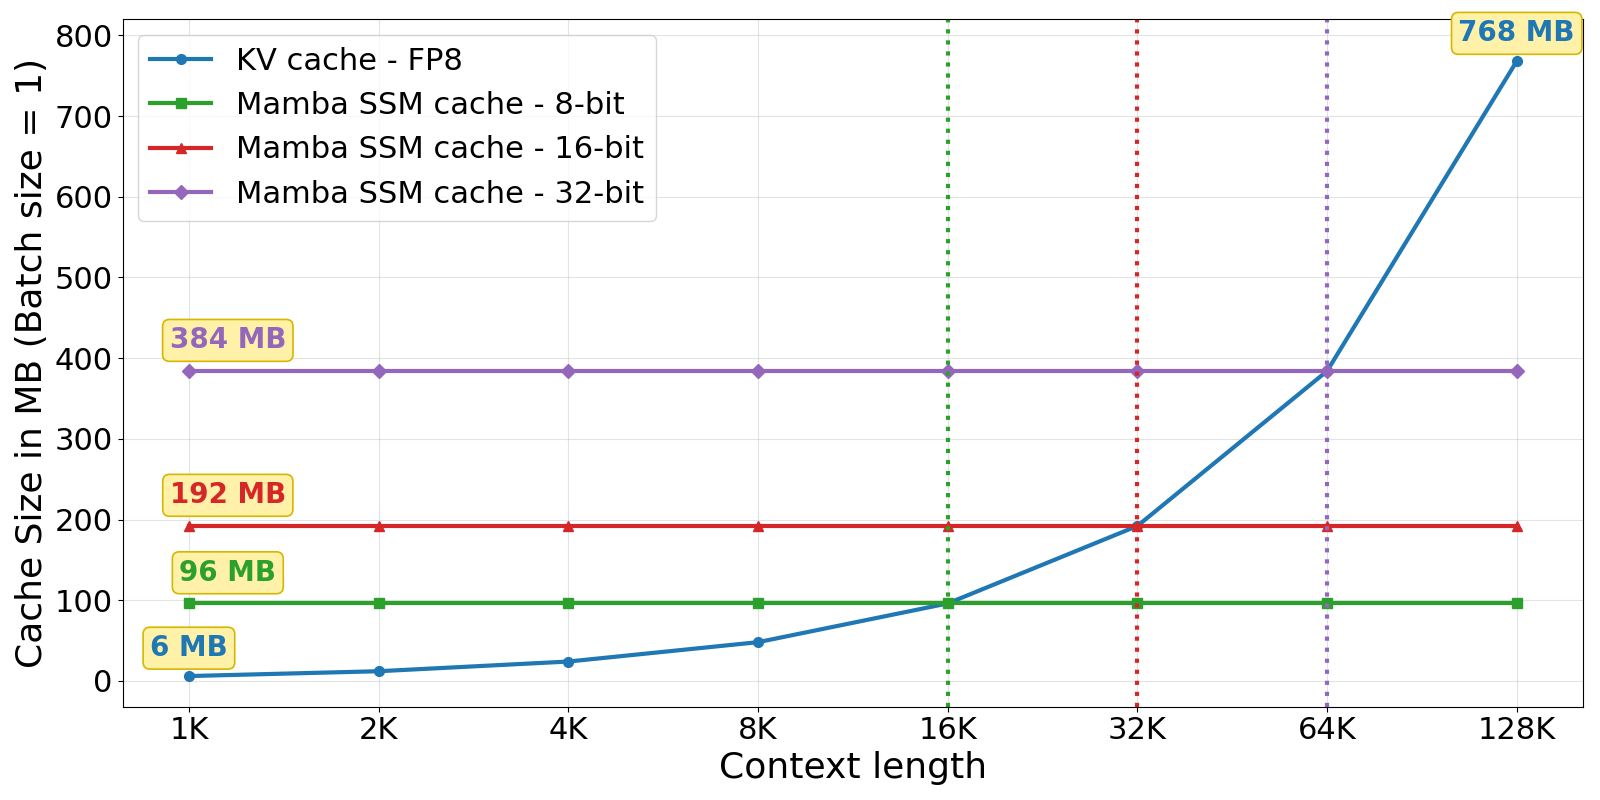
\includegraphics[width=\linewidth]{figures/mamba_vs_kv_cache.png}
\caption{Cache size comparison for FP8 KV cache and Mamba SSM cache at
different cache precisions for batch size 1.}
\label{fig:mamba-vs-kv}
\end{minipage}
\hfill
\begin{minipage}[t]{0.50\linewidth}
\vspace{0pt}
\centering
\scriptsize
\refstepcounter{table}
\label{tab:mamba-cache-quantization}
\setlength{\tabcolsep}{2.5pt}
\renewcommand{\arraystretch}{1.15}
\begin{tabular}{@{}>{\raggedright\arraybackslash}p{0.36\linewidth}
                  >{\centering\arraybackslash}p{0.27\linewidth}
                  >{\centering\arraybackslash}p{0.28\linewidth}@{}}
\hline
\textbf{Mamba cache precision} &
\textbf{Median accuracy drop from FP32 cache} &
\textbf{Average verbosity increase from FP32 cache} \\
% \hline
\midrule
FP16 RTN & 2.32\% & 10.84\% \\
% \hline
FP16 SR & -0.32\% & 1.13\% \\
% \hline
INT8 RTN (block size 128) & 2.87\% & 10.72\% \\
% \hline
INT8 SR,\\ block size = 128 & 0.00\% & 2.03\% \\
% \hline
FP8 RTN,\\ block size = 128 & 12.68\% & 26.07\% \\
% \hline
FP8 SR,\\ block size = 128 & 1.96\% & 3.95\% \\
% \hline
\bottomrule
\end{tabular}
\vspace{0.5em}

\parbox{\linewidth}{\centering\textbf{Table~\thetable:} Mamba cache
quantization results on Nemotron 3 Super. Accuracy and verbosity are measured
based on the following evaluation benchmarks: MMLU Pro, GPQA, HLE, LiveCodeBench, IFBench,
OmniScience, AA-LCR, Ruler 128K, and Ruler 256K. For both metrics, lower is better.}
\end{minipage}
\end{figure}

Therefore, depending on the sequence length and batch size, the Mamba cache can become both a DRAM-footprint bottleneck and a source of DRAM-read pressure that limits decoding speed.

To address this, we quantize the Mamba SSM cache from the original FP32 precision to lower precisions.
Following Nemotron 3 Super~\citep{nvidia2026nemotron3superopen}, we first adopt 16-bit cache precision, where FP16 with stochastic rounding preserves FP32-cache accuracy and verbosity.

To further improve cache compression, we also explore 8-bit Mamba cache quantization formats.
We evaluated this on Nemotron 3 Super and validated that the conclusions hold on Nemotron 3 Ultra. Experimental results on the effect of Mamba cache quantization on Nemotron 3 Super are summarized in Table~\ref{tab:mamba-cache-quantization}.

Consistent with Nemotron 3 Super~\citep{nvidia2026nemotron3superopen}, we find that the mantissa precision and stochastic rounding are key ingredients for preserving accuracy after Mamba cache quantization.
Block-scaled INT8 quantization with stochastic rounding largely preserves FP32-cache accuracy and verbosity. FP8 E4M3 quantization degrades accuracy, likely because it provides lower effective precision for these cache values than INT8.

Optimized INT8 Mamba cache kernels are still under development. For the current
release, we use FP16 SSM cache storage with stochastic rounding, as described in
Nemotron Super~\citep{nvidia2026nemotron3superopen}, which avoids block-scaling overhead while
mitigating the recurrent rounding bias observed with naive FP16 round-to-nearest cache storage.


\subsection{SSM Cache Checkpointing}
To further reduce the quantization error caused by Mamba SSM state caching, we explore the idea of periodic cache checkpointing: Instead of storing (thus, quantizing) the state in each decoding step, we store it every $CC$ steps for an integer $CC>1$. To compensate for the state being behind, we cache the input activations and apply activation replay to forward the state on-the-fly. This reduces the number of sequential quantization steps by a factor of $CC$ and can also save time due to saving on cache writes (though there is a tradeoff with the additional compute and IO used for the activation replay).

We ran initial experiments on Nemotron 3 Super NVFP4, using QDQ gates. The results are summarized in Table~\ref{tab:mamba-cache-checkpointing}.

\begin{table}[!htp]
\centering
\small
\setlength{\tabcolsep}{8pt}
\renewcommand{\arraystretch}{1.3}
\resizebox{\textwidth}{!}{%
\begin{tabular}{@{}>{\raggedright\arraybackslash}p{0.36\linewidth}
                  >{\centering\arraybackslash}p{0.27\linewidth}
                  >{\centering\arraybackslash}p{0.28\linewidth}@{}}
\hline
\textbf{Mamba cache precision} &
\textbf{Mean accuracy drop from FP32 cache} &
\textbf{Average verbosity increase from FP32 cache} \\
% \hline
\midrule
% FP16 RTN                           &  1.07\% &  9.97\% \\
% \hline
% FP16 RTN, CC = 8                   &  0.02\% &  3.02\% \\
% \hline
% FP16 SR                            & -0.26\% &  0.34\% \\
% \hline
% FP16 SR,  CC = 8                   &  0.19\% &  0.34\% \\
% \hline
INT8 RTN, block size = 128           &  2.87\% &  9.85\% \\
% \hline 
INT8 RTN, block size = 128, CC = 8   &  1.14\% &  4.14\% \\
% \hline 
INT8 SR,  block size = 128           & 0.00\% &  1.23\% \\
% \hline
INT8 SR,  block size = 128, CC = 8   & -0.76\% &  0.56\% \\
% \hline
INT8 SR,  block size = 64, CC = 32   & -1.07\% &  0.00\% \\
% \hline
FP8 RTN,  block size = 128           &  12.68\% & 25.08\% \\
% \hline 
FP8 RTN,  block size = 128, CC = 8   &  1.89\% &  3.7\%  \\
% \hline 
FP8 SR,   block size = 128           &  1.96\% &  3.14\% \\
% \hline 
FP8 SR,   block size = 128, CC = 8   &  0.69\% &  1.34\% \\
% \hline
FP8 SR,   block size = 64, CC = 32   &  0.19\% &  0.67\% \\
% \hline
\bottomrule
\end{tabular}
}
\caption{
Mamba cache checkpointing and quantization results on the Nemotron 3 Super NVFP4 model. ``CC'' stands for the period length used for checkpointing. Accuracy and verbosity are measured based on the following evaluation benchmarks: MMLU Pro, GPQA, HLE, LiveCodeBench, IFBench, OmniScience, AA-LCR, Ruler 128K, and Ruler 256K. For both metrics, lower is better.
}
\label{tab:mamba-cache-checkpointing}
\end{table}
\end{comment}

\subsection{SSM Cache Optimization}
\label{sec:ssm-cache-optimization}

In Mamba autoregressive decoding, the SSM state is stored in a
constant-sized cache for each batch element. The KV
cache size, on the other hand, grows with sequence length.
However, there is a crossover point below which the Mamba cache size is larger than the KV cache size.
For example, in Nemotron 3 Ultra, the 32-bit Mamba cache is larger than the FP8 KV cache at sequence lengths up to 64K. This is illustrated in Figure~\ref{fig:mamba-vs-kv}. 

\begin{figure}[t]
\centering
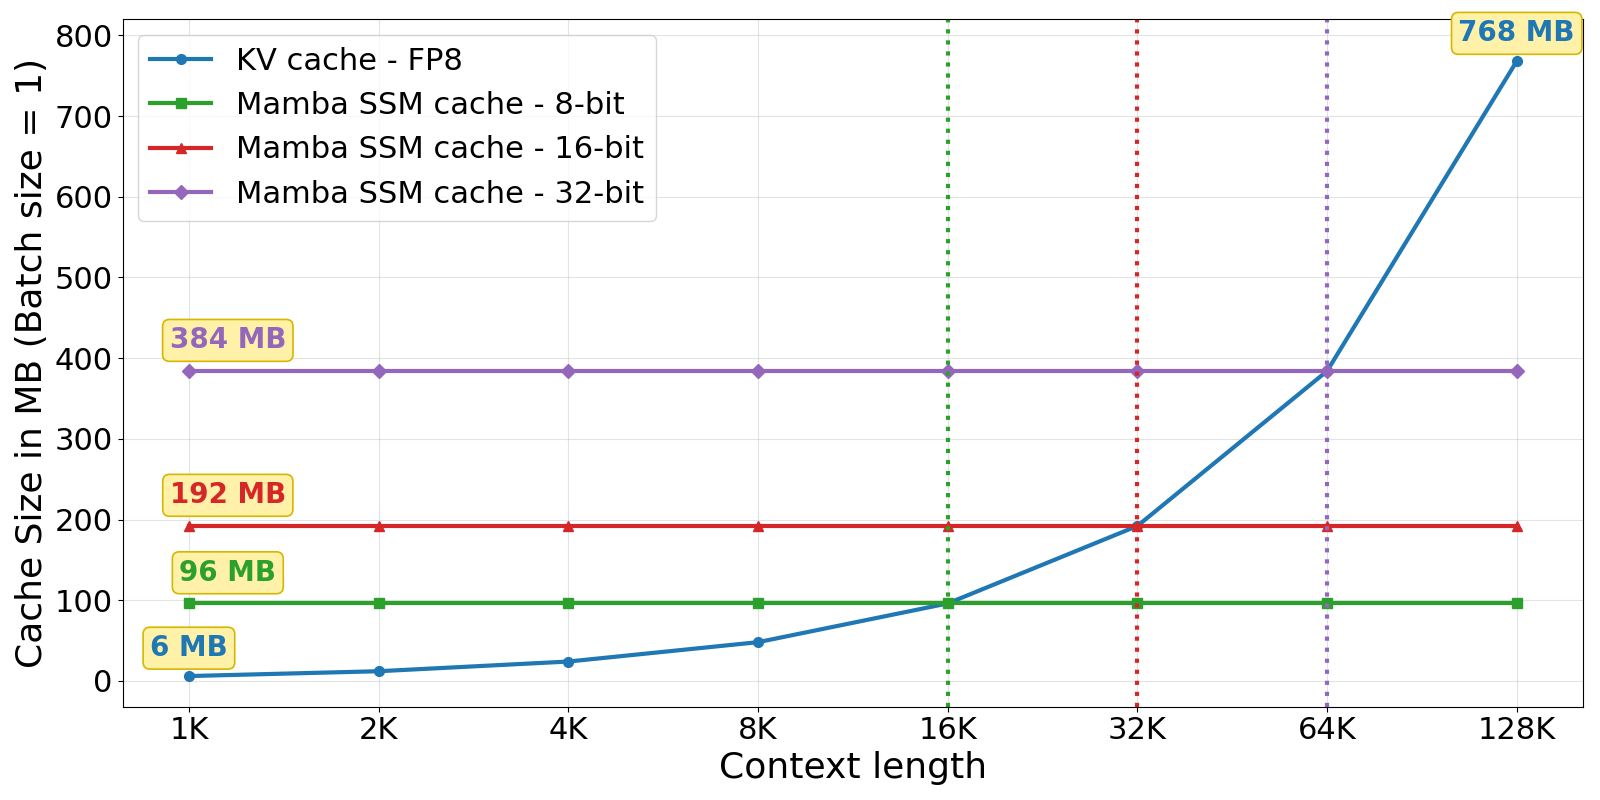
\includegraphics[width=0.72\linewidth]{figures/mamba_vs_kv_cache.png}
\caption{Cache size comparison for FP8 KV cache and Mamba SSM cache at
different cache precisions for batch size 1.}
\label{fig:mamba-vs-kv}
\end{figure}

Therefore, depending on the sequence length and batch size, the Mamba cache can become both a DRAM-footprint bottleneck and a source of DRAM-read pressure that limits decoding speed.

To address this, we quantize the Mamba SSM cache from the original FP32 precision to lower precisions.
Following Nemotron 3 Super~\citep{nvidia2026nemotron3superopen}, we first adopt 16-bit cache precision, where FP16 with stochastic rounding preserves FP32-cache accuracy and verbosity.

To further improve cache compression, we also explore 8-bit Mamba cache quantization formats.
We evaluated this on Nemotron 3 Super.

Consistent with Nemotron 3 Super~\citep{nvidia2026nemotron3superopen}, we find that the mantissa precision and stochastic rounding are key ingredients for preserving accuracy after Mamba cache quantization.
Block-scaled INT8 quantization with stochastic rounding largely preserves FP32-cache accuracy and verbosity. FP8 E4M3 quantization degrades accuracy, likely because it provides lower effective precision for these cache values than INT8.
The Mamba cache quantization results are summarized in Table~\ref{tab:mamba-cache-checkpointing}.

To further reduce the quantization error caused by Mamba SSM state caching, we explore the idea of periodic cache checkpointing: Instead of storing (thus, quantizing) the state in each decoding step, we store it every $CC$ steps for an integer $CC>1$. To compensate for the state being behind, we cache the input activations and apply activation replay to forward the state on-the-fly. This reduces the number of sequential quantization steps by a factor of $CC$ and can also save time due to saving on cache writes (though there is a tradeoff with the additional compute and IO used for the activation replay).

We ran initial experiments on Nemotron 3 Super NVFP4, using emulated quantization. The results are summarized in Table~\ref{tab:mamba-cache-checkpointing}.

\begin{table}[!htp]
\centering
\small
\setlength{\tabcolsep}{5pt}
\renewcommand{\arraystretch}{1.2}
\resizebox{\textwidth}{!}{%
\begin{tabular}{@{}>{\raggedright\arraybackslash}p{0.30\textwidth}
                  *{4}{>{\centering\arraybackslash}p{0.175\textwidth}}@{}}
\toprule
\textbf{Mamba cache precision} &
\multicolumn{2}{c}{\textbf{Quantization (No Checkpointing)}} &
\multicolumn{2}{c}{\textbf{Quantization + Checkpointing (CC = 8)}} \\
\cmidrule(lr){2-3}
\cmidrule(lr){4-5}
&
\textbf{Mean accuracy drop from FP32 cache} &
\textbf{Average verbosity increase from FP32 cache} &
\textbf{Mean accuracy drop from FP32 cache} &
\textbf{Average verbosity increase from FP32 cache} \\
\midrule
FP16 RTN & 1.07\% & 9.98\% & 0.03\% & 3.07\% \\
FP16 SR & -0.26\% & 0.36\% & 0.19\% & 0.40\% \\
INT8 RTN, block size = 128 & 1.42\% & 9.91\% & 0.30\% & 4.16\% \\
INT8 SR, block size = 128 & -0.15\% & 1.28\% & -0.42\% & 0.60\% \\
FP8 RTN, block size = 128 & 4.68\% & 25.17\% & 0.46\% & 3.69\% \\
FP8 SR, block size = 128 & 0.61\% & 3.12\% & 0.29\% & 1.41\% \\
\bottomrule
\end{tabular}
}
\caption{
Mamba cache checkpointing results on the Nemotron 3 Super NVFP4 model with emulated quantization, measured relative to the same model with FP32 Mamba cache. CC denotes the checkpointing period. Accuracy and verbosity are measured based on the following evaluation benchmarks: MMLU Pro, GPQA, HLE, LiveCodeBench, IFBench, OmniScience, AA-LCR, Ruler 128K, and Ruler 256K. For both metrics, lower is better.
}
\label{tab:mamba-cache-checkpointing}
\end{table}

Optimized 8-bit Mamba cache kernels with checkpointing support are under development.
For the current release, we use FP16 SSM cache storage with stochastic rounding, as described in Nemotron Super~\citep{nvidia2026nemotron3superopen}, which avoids block-scaling overhead while mitigating the recurrent rounding bias observed with naive FP16 round-to-nearest cache storage.


\subsection{One NVFP4 checkpoint}

We release a single NVFP4 checkpoint for \ourmodel{} that targets both
Blackwell, where it runs with native FP4 math, and Hopper, where it runs
as W4A16 (weights NVFP4, activations BF16). This is because Hopper lacks native FP4
tensor cores. KV Cache is quantized to FP8 and Mamba cache data type is FP16 with stochastic rounding.

The natural candidate for Hopper would have been a separate FP8 checkpoint to un-lock FP8 tensor-core math.
At first glance W8A8 should be the better Hopper choice: FP8 tensor
cores have higher peak throughput than the BF16 math the W4A16 path
relies on. In practice the opposite holds at \ourmodel's scale. With
TP=8 on an 8-GPU H100 node ($640$~GiB of aggregate HBM), the FP8
checkpoint ($\approx 540$~GiB) leaves roughly $10$~GiB per GPU for
activations, KV cache, and Mamba state, against roughly $40$~GiB for
the NVFP4 checkpoint ($\approx 330$~GiB). The tight FP8 cache budget
caps the maximum batch size at the operating points we care about,
which keeps the workload memory-bandwidth-bound and prevents us from
ever reaching the compute-bound regime where FP8 tensor cores would
matter. The measured throughput-versus-user-latency Pareto places
W4A16 on or above W8A8 across the relevant range.

The case for the single NVFP4 checkpoint becomes much stronger once
MTP is in the picture. The reduced W4 footprint leaves enough headroom
to fit MTP weights on the same 8-GPU node, while the FP8 checkpoint
cannot fit MTP without scaling to two H100 nodes and surrendering the
single-NVLink-domain property. With MTP enabled on the W4A16 path, the
throughput-versus-user-latency Pareto both moves up across the relevant
range and extends much further into the low-latency regime than W8A8
reaches at any operating point.

A third option, W4A8, NVFP4 weights with FP8 activations, would
in principle combine the smaller weight footprint with FP8 tensor-core
math. We chose not to ship it. Naively downcasting NVFP4 weights to FP8
causes catastrophic accuracy degradation: NVFP4 uses E2M1 elements with
E4M3 block scales, giving an effective E6M4 representation whose range
exceeds FP8's E4M3, so the resulting weights saturate. Preserving
accuracy therefore requires a W4 $\rightarrow$ BF16 $\rightarrow$ FP8
round-trip rather than a direct W4 $\rightarrow$ FP8 cast, which adds
an extra cast op before each GEMM. Combined with the result above, 
even pure W8A8 is slower than W4A16 in our regime, the extra op
makes W4A8 strictly worse than W4A16, with no accuracy upside.

\begin{table}[ht!]
\centering
\small
\setlength{\tabcolsep}{5pt}
\renewcommand{\arraystretch}{1.3}

% requires: booktabs
\begin{tabular}{l|cc|cc|cc}
\toprule
& \multicolumn{2}{c|}{\textbf{BF16}}
& \multicolumn{2}{c|}{\textbf{W4A16}}
& \multicolumn{2}{c}{\textbf{NVFP4 (W4A4)}} \\
\cmidrule(lr){2-3} \cmidrule(lr){4-5} \cmidrule(lr){6-7}
\textbf{Task} & \textbf{Score} & \textbf{Tok.}
            & \textbf{Score} & \textbf{Tok.}
            & \textbf{Score} & \textbf{Tok.} \\
\midrule
GPQA           & \textbf{86.67} & 14408 & \textbf{86.67} & 14841 & 86.36          & 15134 \\
HLE            & \textbf{26.92} & 37479 & 25.12          & 39103 & 25.67          & 39103 \\
IFBench        & 82.12          & 5272  & \textbf{82.75} & 5466  & 82.42          & 5764  \\
AA-Omniscience & 24.38          & 1140  & \textbf{25.50} & 1396  & 24.55          & 1226  \\
AA-LCR         & 63.67          & 4110  & \textbf{65.33} & 4286  & 64.00          & 4346  \\
\bottomrule
\end{tabular}
\caption[BF16 vs.\ W4A16 vs.\ NVFP4]{
  Accuracy and verbosity of the single NVFP4 checkpoint deployed as W4A16 (NVFP4
  weights, BF16 activations) and as NVFP4 (W4A4, native FP4; the
  Blackwell path), against the BF16 reference. \textbf{Score} is pass@1; \textbf{Tok.}\
  is the average completion length in tokens. Higher score per task is in bold.
  W4A16 outperforms NVFP4 on four of five tasks (all but HLE), stays within $1$~point
  of or above BF16 on four of five tasks (all but HLE), and produces no more completion
  tokens than NVFP4 on four of five tasks (all but AA-Omniscience).
}
\label{tab:w4a16-vs-nvfp4}
\end{table}

\begin{table*}[!htp]
\centering
\footnotesize
\setlength{\tabcolsep}{2.5pt}
\renewcommand{\arraystretch}{1.05}
\begin{tabular*}{\textwidth}{@{\extracolsep{\fill}}l|c c }
\toprule
\textbf{Benchmark}
& \makecell{\textbf{N-3-Ultra}\\\textbf{BF16}}
& \makecell{\textbf{N-3-Ultra}\\\textbf{NVFP4}}\\

\midrule
\rowcolor{black!5}
\multicolumn{3}{l}{\textbf{Agentic}} \\
\midrule
Terminal Bench 2.1 & 56.4 &  53.9 \\
GDPVal & 46.7 & 47.9   \\
SWE-Bench Verified & 70.7 & 69.5  \\
SWE-Bench Multilingual & 67.7 & 69.1  \\
ProfBench (Search) & 56 & 56.4 \\
PinchBench & 90 & 89.8  \\
TauBench V3 & &   \\
\quad Airline & 81.5 & 80.0 \\
\quad Retail  & 86.4 & 88.4 \\
\quad Telecom & 92.9 & 93.6 \\
\quad Banking & 22.6 & 19.2 \\
\quad Average & 70.9 & 70.3 \\
BrowseComp & 44.4 & 41.4 \\

\midrule
\rowcolor{black!5}
\multicolumn{3}{l}{\textbf{Reasoning and Knowledge}} \\
\midrule
IOI 2025 & 570.0 & 564.7 \\
GPQA (no tools) & 87.0 &  87.9 \\
SciCode (subtask) & 44.6 & 43.5   \\
HLE (no tools) & 26.7 & 26.1   \\
CritPt (no tools) & 3.1 & 3.4  \\
OmniScience Accuracy & 24.1 & 24.6  \\
OmniScience Non-Hallucination & 78.7 & 75.5 \\

\midrule
\rowcolor{black!5}
\multicolumn{3}{l}{\textbf{Chat \& Instruction Following}} \\
\midrule
IFBench (prompt) & 81.7 & 82.3  \\

\midrule
\rowcolor{black!5}
\multicolumn{3}{l}{\textbf{Long Context}} \\
\midrule
AA-LCR & 65.4 & 65.5  \\
RULER 1M & 94.7 & 94.0  \\

% \midrule
% \rowcolor{black!5}
% \multicolumn{3}{l}{\textbf{Multilingual}} \\
% \midrule
% MMLU-ProX (avg over langs) & &  \\
% WMT24++ (en$\rightarrow$xx) & &  \\

\bottomrule
\end{tabular*}

\caption{
Evaluation suite comparing BF16 and NVFP4 of \ourmodel. BF16 uses vLLM 0.17.1, NVFP4 uses vLLM 0.22.0.
}
\label{tab:super_comparison}
\end{table*}
